\chapter{Deploy dei modelli ML}

Una volta che è stato effettuato correttamente il training e la creazione di un modello
machine learning, arriva il momento di distribuirlo e di utilizzarlo effettivamente
per il suo scopo, ovvero quello di classificatore di tipi di parcheggio.\\
L'idea generale del funzionamento consiste nel raccogliere dati durante il tragitto
dell'auto e in seguito fornirli come input al modello. Chiaramente, i dati che 
il modello prodotto riceve in input devono essere della stessa forma di quelli
utilizzati per fare il training. Ciò implica che tutte le procedure di pulizia
dei dati e di miglioramento delle feature debbano essere ripetute ogni volta che
nuovi dati vengono raccolti per essere sottoposti al modello ed essere 
classificati.\\
Garantire che un modello riceva in input dati di forma e qualità identiche a
quelle del dataset di training può talvolta risultare laborioso. Ciò è causato 
dal fatto che gli ambienti di raccolta dati e quelli di produzione possono 
differire sotto svariati aspetti. Infatti, non è scontato che in queste due
situazioni si utilizzino lo stesso linguaggio di programmazione, lo stesso sistema
operativo, le stesse librerie, gli stessi approcci, ecc. Al contrario, è
molto probabile che un modello venga istruito una volta, per poi essere 
distribuito ed utilizzato su piattaforme diverse. In queste situazioni si può
andare incontro a numerose complicazioni, come dover ri-progettare alcuni
algoritmi a causa di un cambiamento di linguaggio di programmazione, che 
renderebbe l'algoritmo stesso meno efficente o addirittura non più funzionante.
In questo caso, è fondamentale avere una conoscenza approfondita del funzionamento
dell'algoritmo originale e della buona documentazione da poter consultare. 
Qualsiasi minimo errore di trascrizione o di comprensione potrebbe generare
modifiche sostanziali ai dati che verranno processati, rendendoli così differenti
da quelli provenienti dal training set e non più validi per una potenziale
classificazione. Spesso si può anche andare incontro ad un cambiamento di librerie,
soprattutto se si sta cambiando linguaggio di programmazione. La questione che
riguarda le librerie è ancora più delicata rispetto a quella dei linguaggi. Nella
maggior parte dei casi, esse contengono delle logiche interne che risultano molto
complesse da riprodurre o imitare in un ambiente differente. Per questo motivo,
è bene ridurre al minimo l'utilizzo di librerie esterne quando ci si trova in 
situazioni come questa, ovvero scrivendo codice che dovrà essere portato su altre
piattaforme. Tuttavia, a volte è necessario utilizzare alcune librerie, come nel
nostro caso, in cui si sono dovute utilizzare libreria per l'algebra lineare.
Quindi, anche per questo discorso occorre avere massima prudenza nella scelta di
un sostituto valido e che non generi inconsistenze nei dati.

\section{Necessità del calcolo in locale}

Per quanto riguarda il deploy di un modello, un'altra scelta da prendere è se 
eseguire il modello in un applicativo lato client, oppure su un server remoto.
Questa decisione dipende da molti fattori, tra i quali vi è la potenza di calcolo
del dispositivo che esegue l'applicativo client, potenziali requisiti di esecuzione
real-time (con bassa latenza), disponibilità del dispositivo di una connessione 
ad internet, sensibilità dei dati, ecc.\\
Entrambi gli approcci hanno vantaggi e svantaggi. Tra i vantaggi di una
 esecuzione lato server possiamo notare: 
\begin{itemize}
    \item la possibilità di sostituire il modello con una versione più aggiornata
    senza dover per forza rilasciare un nuovo aggiornamento dell'applicativo client
    \item poter effettuare l'esecuzione di un modello al posto di un dispositivo
   	con scarsa potenza di calcolo (es. un dispositivo embedded) \cite{computation_offloading_ml}
\end{itemize}
Invece tra quelli di una esecuzione lato client:
\begin{itemize}
    \item non dover dipendere da un server remoto, quindi da una connessione 
    stabile 
    \item evitare di dover attendere una risposta dal server, che può impiegare
    molto più tempo che una esecuzione in locale (nel caso in cui la potenza di
    calcolo del dispositivo sia sufficente)
    \item mantenere privati i dati che sono utilizzati come input del modello
    (nel caso in cui i dati siano sensibili)
\end{itemize}
Nel caso del nostro modello, è stato deciso di eseguire la predizione del modello
in locale, nel lato client dell'app GeneroCity. Questa scelta è stata presa 
principalmente per due motivi:
\begin{itemize}
    \item in prospettiva di un utilizzo dell'app da parte di numerosi utenti,
    evitare che il server backend venga sottoposto a un carico troppo oneroso,
    causato dalla potenziale esecuzione di un numero molto elevato di 
    classificazioni in parallelo;
    \item sfruttare il \emph{Neural Engine} \cite{mobile_machine_learning_arm} dei 
    dispositivi Apple, attraverso la libreria \emph{Core ML}\footnote{
    \emph{Core ML} page on Apple's website: 
    \href{https://developer.apple.com/documentation/coreml}{\underline{link to the page.}}} 
    \cite{introduction_core_ml} (solamente per la versione iOS di GeneroCity);
\end{itemize}

Dal momento che il processo di classificazione, attraverso un modello, è 
abbastanza intensivo e inoltre richiede la pulitura dei dati preliminare,
permettere che venga eseguito su un server potrebbe generare rallentamenti.
Questo si verifica soprattutto se il programma backend non è distribuito.
Oltre a ciò, vi è il fatto che l'esecuzione del modello avviene in seguito
ad un'azione dell'utente (ovvero al parcheggio dell'auto) e nel caso in cui 
ci fossero degli utenti malintenzionati, si correrebbe il rischio di
ricevere troppe richieste allo stesso tempo.

\subsection{Predizione in locale con Core ML}

Dovendo effettuare la classificazione in locale, su piattaforma iOS, la 
libreria che è risultata più adatta ai nostri scopi è stata \emph{Core ML}.
Questa libreria da la possibilità di integrare modelli machine learning 
direttamente all'interno delle app. Oltre a fornire dei modelli già 
addestrati e pronti all'uso (tra cui uno per il riconoscimento di immagini,
un altro per la trascrizione audio-testo, ecc.), essa offre dei modi per 
utilizzare modelli creati direttamente dallo sviluppatore.\\
Innanzitutto, \emph{Core ML} richiede che i modelli proposti dallo
sviluppatore siano del formato proprietario ".mlmodel". Questo formato,
infatti, è stato creato proprio da Apple. Ci sono principalmente due 
modi per ottenere un modello di questa tipologia:
\begin{itemize}
    \item crearlo direttamente attraverso la libreria \emph{Create ML};
    \item convertirne uno di un altro formato (es. TensorFlow\footnote{
    TensorFlow's website: 
    \href{https://www.tensorflow.org}{\underline{link to the page.}}}) attraverso 
    un apposito strumento di conversione, che fa parte della libreria Python
    \emph{coremltools\footnote{
    \emph{coremltools} page on GitHub: 
    \href{https://apple.github.io/coremltools/}{\underline{link to the page.}}}};
\end{itemize}
Siccome per iniziare è stato integrato il modello soltanto nella versione
iOS dell'app, è stata scelta la prima strada, ovvero generarlo con
\emph{Create ML} (Figura~\ref{fig:flow_diagram_deploy_modello}). 
In questo modo non è stato necessario utilizzare
strumenti più personalizzabili, ma molto più complessi e a basso
livello, come TensorFlow.\\
La scelta di \emph{Core ML} è stata ovvia, in quanto su iOS è l'unica
libreria che permette di sfruttare al meglio l'hardware del dispositivo.
Infatti, essa è stata progettata proprio per essere utilizzata in
accoppiata con l'hardware GPU presente negli stessi dispositivi Apple.
Inoltre, nei dispositivi delle generazioni più recenti è stato inserito
un componente dedicato esclusivamente all'esecuzione di algoritmi di
intelligenza artificiale e modelli ML, chiamato \emph{Neural Engine}.
Esso si tratta di una sezione del SoC del dispositivo, che è provvista di una 
architettura ad hoc e che viene sfruttata quando vengono invocate delle
predizioni attraverso \emph{Core ML}. Questa sezione è stata aggiunta 
a causa di una presenza del machine learning all'interno delle app
che è aumentata drasticamente negli ultimi anni e che con ogni
probabilità continuerà a diffondersi. Grazie a questo componente,
l'esecuzione di una predizione di machine learning (es. la 
classificazione del tipo di parcheggio) non va ad influire sulle
performance del sistema (sul resto dell'hardware) e quindi non 
crea rallentamenti o problemi visibili dall'utente.\\
Avendo deciso di eseguire il modello in locale, diventa obbligatorio
effettuare anche le fasi preliminari di preparazione dei dati in 
locale. Quindi, l'intera procedura, che va dal parcheggio 
dell'auto fino alla predizione del tipo di parcheggio, viene
eseguita all'interno dell'app iOS, senza alcun sostegno di 
servizi esterni.
\begin{figure}
    \centering
    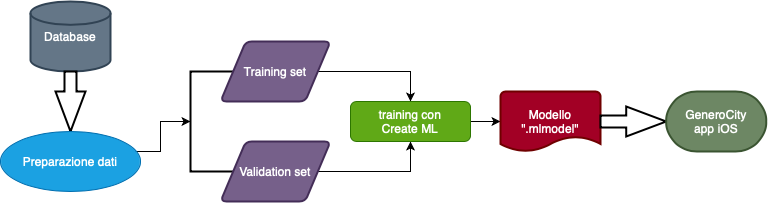
\includegraphics[width=14cm]{images/flow_diagram_deploy_modello.png}
    \caption{Diagramma di flusso del deploy del modello.}
    \label{fig:flow_diagram_deploy_modello}
\end{figure}

\section{Porting del processore di dati}

Come già anticipato, la scelta di eseguire la classificazione del tipo di
parcheggio in locale nell'applicazione implica delle conseguenze.
Una delle più importanti tra queste è certamente il fatto di dover
pulire e preparare i dati direttamente in ambiente iOS. Ciò
ha reso obbligatorio un porting dello script dedicato a processare i
dati delle registrazioni, che è scritto in Python. Il linguaggio di 
destinazione del porting è Swift\footnote{
Swift's website: 
\href{https://swift.org}{\underline{link to the page.}}}, ovvero il linguaggio utilizzato
per sviluppo di GeneroCity iOS.

\subsection{Da Python a Swift}

Python e Swift differiscono sotto molti aspetti: oltre ad avere una sintassi
significativamente diversa, sono stati progettati per scopi abbastanza 
differenti e i loro ambienti di esecuzione non hanno molti fattori 
in comune. Mentre Python è pensato per essere utilizzato su una vasta
varietà di sistemi operativi e architetture, offrendo un interprete
con ampia compatibilità, Swift ha una target più ristretto, che 
mira principalmente ai dispositivi con sistemi operativi Apple.
Tuttavia, la differenza maggiore sta nel fatto che Python si tratta
di un linguaggio interpretato, mentre Swift è un linguaggio compilato. 
Il secondo, quindi, ha bisogno di un compilatore apposito (ovvero \emph{Swiftlang} 
e \emph{LLVM} \cite{llvm_clang}) che generi
i binari che infine vengono eseguiti.\\
Essendo due linguaggi molto utilizzati e con un background notevole,
entrambi sono dotati di un solida fornitura di librerie. Infatti, 
considerando sia librerie native, che librerie di terze parti,
Python e Swift possono essere sfruttati in moltissimi ambiti.
Per quanto riguarda il nostro obiettivo, è stato necessario
utilizzare operazioni di algebra lineare e fortunatamente entrambi i
linguaggi sono muniti di librerie mature abbastanza da permettere di 
svolgere tali operazioni in maniera sufficentemente intuitiva.\\
Ad ogni modo, la trascrizione del codice stesso non è stata affatto
priva di complicazioni. Sono state notate numerose differenze tra i
linguaggi, che hanno reso il porting una operazione tutt'altro che 
lineare:
\begin{itemize}
    \item \textbf{strutture sintattiche}: i due linguaggi differiscono alla base,
    nel modo di gestire gli scope dei blocchi di codice (python utilizza
    l'indentazione, mentre Swift utilizza uno stile a parentesi graffe
    C-like) e in molte strutture, come le dichiarazioni di cicli, 
    esecuzioni condizionali, operatori booleani, ecc.
    \item \textbf{presenza di variabili e costanti}: Swift necessita che venga 
    specificata l'entità di una variabile (se si tratta di una variabile
    o di una costante) al momento della sua dichiarazione, mentre in Python
    sono già tutte semplici variabili di default. Inoltre Swift permette
    di aggiungere molte altre keyword (es. modificatori di accesso) alle
    dichiarazioni di variabili, in modo modificare le loro proprietà.
    \item \textbf{tipizzazione}: mentre Python appartiene al gruppo di linguaggi
    tipizzati dinamicamente (ovvero, che permettono ad una stessa
    variabile di assumere tipi diversi all'interno dello stesso scope
    di esecuzione), Swift è tipizzato staticamente (cioè, non permette
    che una variabile cambi il proprio tipo, nello stesso scope, durante
    una esecuzione). Questo implica anche che in molti contesti, in Swift,
    bisogni esplicitamente definire il tipo richiesto (ad esempio nella
    dichiarazione dei parametri e del valore di ritorno di una funzione),
    a differenza di Python, in cui il tipo non viene mai definito. 
    \item \textbf{strutture dati}: non è immediato riportare molte strutture ad alto 
    livello che si trovano su Python (es. la \emph{List}) su un linguaggio
    come Swift. Spesso è necessario avere delle accortezze maggiori per 
    gestire dei dati ad un livello leggermente più basso rispetto a come 
    venivano gestiti su Python. Inoltre, il formato JSON che nel nostro 
    script è stato ampiamente utilizzato, viene mappato direttamente 
    a strutture dati Python, mentre richiede delle conversioni più
    mirate all'interno di Swift.
    \item \textbf{passaggi di argomenti a funzioni per riferimento e per valore}:
    i due linguaggi differiscono in alcuni casi nel passaggio di parametri a 
    funzioni. Infatti, per strutture come gli array, Python non crea copie
    al momento del passaggio di un'istanza come argomento ad una funzione.
    Quindi, all'interno dello scope della funzione si ha accesso al 
    riferimento della struttura iniziale e ogni modifica applicata ad
    essa rimarrà persistente anche quando l'esecuzione della funzione sarà 
   	terminata. Al contrario, questo tipo di strutture sono passate in 
   	Swift come valore, ovvero, vengono create delle copie al momento della
   	chiamata di funzione. Questo significa che tutte le azioni effettuate
    su una determinata struttura di questo tipo, dopo essere stata copiata, 
    non andranno a coinvolgere la copia originale. Inoltre, di default, Swift
    istanzia le variabili passate come argomento di funzione come "let",
    ovvero costanti, e quindi non permette modifiche.
    \item \textbf{gestione delle variabili opzionali}: mentre Python utilizza un
    approccio più classico a riguardo, Swift fornisce un sistema
    abbastanza sofisticato per la gestione delle variabili opzionali,
    al fine di tutelare il programmatore nel ridurre il numero degli errori
    dovuti alla presenza di valori nulli all'interno delle variabili.
    Di fatto, a causa della natura di linguaggio interpretato e della
    tipizzazione dinamica, Python non segnala potenziali problemi scaturiti
    da chiamate di funzioni su una variabile nulla e quindi semplicemente 
    genera un'eccezione a tempo di esecuzione. Differentemente, Swift
    introduce il concetto di tipo opzionale \cite{empirical_study_usage_swift}. 
    Un tipo opzionale (sintatticamente
    con lo stesso nome del corrispettivo tipo normale, ma seguito da "?") consiste 
    in un tipo le cui variabili possono contenere un valore nullo. Questo implica
    che i tipi non opzionali di Swift non possono assolutamente trattare 
    valori nulli. Dunque, esistono alcuni operatori che vengono utilizzati
    per assicurare che una variabile opzionale risulti effettivamente in un 
    valore non nullo. Alcuni di questi sono: "!" che consiste in un'asserzione
    (ovvero, garantisce che il contenuto della variabile sia non nullo, a costo 
    di generare un'eccezione se questo non è vero), "?? default" che permette
    di fornire un valore di default nel caso in cui la variabile contenga un 
    valore nullo, ecc. Utilizzare "!" è stato definito come "unwrap", ovvero
    l'azione di "scartare" metaforicamente una variabile, al fine di ottenere
    il vero valore che è "incartato" al suo interno. Potenzialmente, si 
    potrebbe applicare l'unwrap in ogni caso, per ottenere un comportamento 
    simile a quello di Python, ma ciò andrebbe contro le linee guida del
    linguaggio. \\
    I tipi opzionali si possono incontrare spesso all'interno di Swift, come 
    quando si utilizzano dizionari, che potrebbero avere o non avere un valore
    corrispondente ad una chiave. Per di più, è importante saper applicarli
    nel modo corretto. Ad esempio, la segnatura di una funzione deve 
    necessariamente specificare se un suo argomento o il suo valore di 
    ritorno abbia un tipo classico o opzionale.\\
    Il controllo del rispetto di queste regole, all'interno di un programma,
    viene fatto a tempo di compilazione.
    
\end{itemize}

\subsection{Corrispondenza tra le due versioni}

Durante il processo di porting, è stato tenuto un occhio di riguardo per quanto
riguarda la corrispondenza tra la versione originale dello script (in Python) e 
quella in Swift. Ovvero, si è cercato di mantenere i due script il più simili 
possibile, senza stravolgere completamente la struttura del programma. Oltre
a ridurre il rischio che i comportamenti di questi due subiscano delle differenze,
l'importanza di questa accortezza proviene dal fatto che in futuro potrebbero
venire applicate delle modifiche alla copia originale e quindi queste si dovranno
rispecchiare nella versione scritta in Swift. Nel caso in cui il programma venisse
totalmente riprogettato, si perderebbe la corrispondenza tra le due versioni e 
quindi una modifica sostanziale nella versione originale, richiederebbe un grande
lavoro di adattamento nella versione scritta in Swift.

\section{Adattamento all'ambiente mobile (iOS)}

Per portare a termine il porting dello script di preparazione dei dati,
è stato necessario compiere diversi passi. Sono state applicate una serie 
di modifiche, tenendo conto di tutte le differenze tra i due linguaggi 
e ambienti di programmazione che sono state descritte in precedenza.
In situazioni particolarmente delicate, in cui il dislivello tra i due
linguaggi impediva la trascrizione diretta, non si ha potuto far altro
che riprogettare qualche piccola funzione, mantenendo l'opportuna 
cautela.

\subsection{Modifica della sintassi}

Per prima cosa, è stato utile ricostruire il corpo dello script, ovvero 
tutte le funzioni principali, modificando la sintassi di base. Sostanzialmente, 
sono stati modificati gli scope di Python basati su indentazione, in scope
C-like, formati da parentesi graffe. Inoltre, sono state modificate tutte le
condizioni presenti nelle intestazioni dei cicli e di altri costrutti. Esempi
sono l'operatore "and" che diventa "\&\&" e "for i in range(n)" che diventa
"for i in 0..<n".

\subsection{Dichiarazione delle variabili}

Dato che nello script di partenza non appariva alcuna dichiarazione di varibile,
ma soltanto assegnamenti, è stato necessario aggiungerle da zero, in modo da 
adattarsi alla sintassi di Swift. Come procedimento generale, è stato deciso
di rendere costanti (utilizzando la keyword "let") tutte le variabili che 
che contenevano i parametri immutabili, inseriti manualmente nello script.
Invece, è stata utilizzata la semplice keyword "var" per tutte le variabili 
rimanenti, ad eccezione di quelle che rimanevano immutate, con le quali è 
convenuto quindi utilizzare "let". Inoltre, dato che lo script era composto 
da più funzioni modulari che venivano invocate da una singola funzione di
interfaccia, è stata aggiunta la keyword "private" a tutte queste funzioni,
al fine di rendere l'interazione con il nuovo modulo meno incline ad errori.

\subsection{Aggiunta di tipi espliciti}

Sempre al fine di mantenere il codice simile tra le due versioni dello script,
si è fatto un forte utilizzo dell'inferenza di tipo fornita da Swift. Quindi,
ove possibile non si è specificato il tipo nella dichiarazione di variabili.
Tuttavia, è stato obbligatorio specificare il tipo in molti contesti, come
nella segnatura delle funzioni e nella dichiarazione di variabili, senza 
assegnazione diretta. A causa del fatto che Python non rende esplicito
il tipo delle variabili, nel porting si è dovuto gestire caso per caso,
facendo controlli accurati sull'entità di ogni variabile utilizzata.

\subsection{Mappatura delle strutture dati}

La questione delle strutture dati è stata abbastanza delicata, non tanto
per le strutture semplici, ma per quelle più complesse, che sono 
organizzate diversamente all'interno dei due linguaggi.\\
In Python si può sfruttare una libreria nativa per convertire dati in 
formato JSON direttamente in strutture del linguaggio (dizionari, liste, ecc.).
In Swift esiste una libreria di terze parti, chiamata \emph{SwiftyJSON\footnote{
SwiftyJSON repository on GitHub: 
\href{https://github.com/SwiftyJSON/SwiftyJSON}{\underline{link to the page.}}}}, che
ha un comportamento simile a quella di Python, ma con differenze dovute alla
presenza dei tipi opzionali nel linguaggio. Per mantenere il codice Swift, simile
a quello Python, è stata utilizzata \emph{SwiftyJSON} per creare una struttura a 
dizionario "[String : [Double]]" che potesse essere utilizzata per manipolare i 
dati JSON di una registrazione. La chiave di tipo "String" contiene il timestamp,
mentre valore come array di "Double" è la lista dei valori ottenuti dai sensori in 
quell'istante. 

\subsection{Adattamento del passaggio di argomenti}

Per quanto riguarda tutti i parametri delle funzioni che appartenevano a tipi 
primitivi, la trascrizione è stata diretta e pressocché priva di complicazioni.
Invece, non è stato altrettanto semplice gestire parametri di tipi più complessi,
come i dizionari. Infatti, in questo caso è stato riscontrato il problema della
differenza di modalità in cui vengono passati gli argomenti alle funzioni. 
Mentre Python tratta i dizionari come una sorta di oggetto e quindi li 
passa con un riferimento, Swift li tratta come delle struct (simili a quelle 
esistenti in C) e al momento del passaggio genera una vera e propria copia.\\
All'interno dello script originale, sono state apportate modifiche al dizionario
contenente i dati della registrazione, proveniente dal formato JSON. Tutta la
pulizia e la preparazione dei dati sono state fatte principalmente in questo
modo. Dato che le modifiche effettuate sui dati hanno raggiunto un numero 
abbastanza elevato, lo script Python è stato suddiviso in funzioni modulari,
in modo da far applicare una sola modifica ad ogni funzione. Per la maggior parte
dei casi, queste funzioni possono essere definite come procedure, in quanto operano 
sui dati come side effect, senza restituire alcun risultato. La maniera più semplice
e intuitiva di fare ciò è stata quella di passare il dizionario dei dati a tutte le
funzioni. Facendo così, ogni funzione ha potuto lavorare direttamente sull'oggetto 
e applicare modifiche allo stesso.\\
Trasferendo questa logica su Swift direttamente, non si sarebbe ottenuto il risultato 
desiderato. Oltre al fatto che all'interno di ogni funzione sarebbe esistita solamente 
una copia locale del dizionario e quindi nessuna modifica sarebbe stata portata a termine 
alla fine del processo, la differenza più proibitiva sarebbe stata che di default Swift
istanzia le variabili provenienti dagli argomenti di una funzione come costanti,
impedendo così la loro modifica. Quindi, una potenziale opzione
sarebbe stata quella di restituire il dizionario modificato come valore di ritorno della 
funzione e aggiornare la variabile nello scope chiamante, ma per mantenere consistenza 
con lo script originale, si è scelta un'altra strada. Swift offre un modo di passare
argomenti ad una funzione attraverso un riferimento modificabile. Questo meccanismo
richiama un po' il passaggio di puntatori che esiste in C. In questa maniera, è 
possibile modificare direttamente il dizionario all'interno delle funzioni, mantenendo
il side effect come si faceva nello script in Python. Per rendere questo possibile, si
deve specificare nella segnatura, che i parametri della funzione siano di tipo "in-out" e 
precedere la variabile passata come argomento con il simbolo "\&", per forzare il passaggio
per riferimento (similmente a come si farebbe in C).


\subsection{Gestione dei tipi opzionali}

Come già anticipato, Swift incentiva l'utilizzo di tipi opzionali qualora una certa 
variabile potesse avere valore nullo. Questo avviene sempre con i dizionari, in quanto
potrebbe accadere che ad una specifica chiave non sia associato alcun valore. Dato che
nello script si è fatto un frequente utilizzo del dizionario contenente i dati della
registrazione, questa questione si è presentata spesso. Nel caso di questo dizionario,
le chiavi in questione corrispondevano ai timestamp del campionamento, quindi si 
aveva una certezza riguardo l'esistenza delle stesse e dunque è sempre stato possibile 
eseguire l'unwrap forzato dei valori, senza dover forinire un valore di default.
In qualche altra situazione un po' più delicata, è convenuto invece selezionare un
valore di default per garantire un funzionamento corretto nei casi estremi di presenza
di valori nulli. 

\subsection{Sostituzione delle librerie}

Trovandosi con Swift e su un sistema operativo mobile, l'intero ecosistema di librerie
e funzionalità che sfruttava lo script originale, scritto in Python, non può essere
acceduto. Questo implica una necessità di adattamento verso il nuovo ambiente. 
Alcune librerie che venivano utilizzate dallo script originale non sono più
necessarie, grazie a delle differenze nel comportamento dei due programmi.
Altre, invece, sono rimaste necessarie per il corretto funzionamento dello script e 
quindi sono state rimpiazzate da opportune librerie Swift.\\
Dato che il programma originale doveva lavorare su tutte le registrazioni di dati 
effettuate dagli utenti, faceva largo utilizzo del file system per leggere e scrivere 
tutti i dati in una struttura di directory dedicata. Per questo venivano utilizzate
delle librerie di Python per l'interazione con il file system stesso. Nel caso di 
Swift, queste non sono state necessarie, in quanto il processo avviene soltanto 
sui dati di una singola registrazione, e non serve quindi salvare questi su memoria
di archiviazione. Infatti, essi vengono caricati nel database e processati in locale
immediatamente dopo che la raccolta abbia terminato.\\
Tra le vere e proprie azioni applicate sui dati, è capitato spesso di dover utilizzare 
operazioni di algebra lineare, o più in generale, operazioni sofisticate sui numeri.
Nello script Python è stata scelta la libreria esterna \emph{NumPy\footnote{
NumPy's website: 
\href{https://numpy.org}{\underline{link to the page.}}}} \cite{guide_numpy},
in quanto dotata
di tutte le funzionalità da noi richieste. Degli esempi di usi che ne sono stati fatti 
ci sono le rotazioni 3D utilizzando matrici, calcoli di prodotti tra matrici, calcoli 
di deviazioni standard, ecc. Chiaramente queste tipologie di operazioni sono rimaste
presenti nel programma Swift e quindi è stata fatta una ricerca di librerie sostitutive 
che potessero rimpiazzare \emph{NumPy}. Per quanto riguarda le operazioni su vettori 
e matrici \cite{simd_vector_operations}, è stata trovata ed utilizzata la libreria 
\emph{SIMD\footnote{SIMD page on Apple's website: 
\href{https://developer.apple.com/documentation/accelerate/simd}{\underline{link to the page.}}}}, sviluppata 
direttamente da Apple. Questa libreria offre una vasta varietà di funzionalità
riguardanti l'algebra lineare, infatti è stato possibile utilizzarla per definire
matrici, effettuare dot e cross product, applicare normalizzazioni, ecc.
% TODO: maybe add here code snippets of the use of the two libraries from Python and Swift
Per funzioni matematiche più semplici, è stato trovato in Swift un supporto 
diretto, a differenza di Python che ha richiesto l'uso di altre librerie.

\section{Uso del modello nell'app}

Una volta che sono stati preparati i dati, questi sono pronti per essere passati
come input al modello, quindi viene qui descritta l'interazione con esso.

\subsection{Inserimento del modello nell'app}

Per poter effettuare una predizione in locale nell'app, è chiaramente necessario che 
il modello classificatore venga inserito nell'app stessa. Attraverso lo strumento di 
creazione del modello, si è potuto estrarre il modello addestrato, compattato in un 
solo file con estensione ".mlmodel". Per effettuare il deploy di questo file nell'app,
è bastato soltanto aggiungerlo al progetto Xcode\footnote{
Xcode page on Apple's website: 
\href{https://developer.apple.com/xcode/}{\underline{link to the page.}}} e utilizzare l'API fornita 
appositamente da \emph{Core ML}. Infatti, una volta che si ottiene il modello in quel
formato, esso può essere sfruttato completamente attraverso questa libreria.
\emph{Core ML} si occupa della generazione automatica di una serie di classi che 
permettono allo sviluppatore di interagire con il modello. In particolare, fornendo
un modello chiamato "ModelloEsempio.mlmodel", verranno generate le seguenti classi:
\begin{itemize}
    \item "ModelloEsempio": classe utilizzata per l'istanziazione del modello nel
    codice, utilizzata per avviare la predizione.
    \item "ModelloEsempioInput": classe utilizzata per fornire l'input a "ModelloEsempio",
    contiene un costruttore con dei parametri autogenerati, uno per ogni feature di
    input del modello (con il relativo tipo).
    \item "ModelloEsempioOutput":  classe utilizzata ricevere l'output di una predizione
    di "ModelloEsempio". Contiene degli attributi autogenerati (variabili a seconda della
    tipologia di modello), tra cui la feature di output del modello (con il relativo tipo)
    e l'accuratezza della predizione.
\end{itemize}

\subsection{Esecuzione delle predizioni}

Le predizioni effettuate con il modello vengono eseguite subito dopo che l'auto viene 
parcheggiata (Figura~\ref{fig:flow_diagram_predizione_tipo}). Questo è possibile perchè gli unici dati che sono necessari
al modello
sono quelli raccolti durante la guida e fino al momento del parcheggio. In questo modo,
la procedura può essere intrapresa non appena viene chiamato il metodo \emph{Car.park()}.
Dato che all'interno di \emph{Car.park()} veniva effettuata già una chiamata a 
\emph{ParkTypeSampleCollector} per l'interruzione della raccolta dati, si è pensato di 
integrare la predizione direttamente nella classe del raccoglitore e lanciarla subito
dopo la terminazione della raccolta. A questo fine, è stato definito un metodo privato
del raccoglitore, chiamato \emph{inferType()}. Questo metodo ritorna un \emph{ParkType},
ovvero il risultato della predizione.\\
All'interno di \emph{inferType()}, la prima cosa che avviene è la la preparazione dei 
dati. Questo significa che viene presa la struttura JSON con i dati appena raccolti e 
passata all'algoritmo definito in precedenza, che effettua tutte le operazioni necessarie
sui dati. Una volta che si hanno i dati processati, è possibile generare l'input per il 
modello. % TODO: maybe specify structure of the input
Vengono estratte dai dati le feature necessarie per il modello e passate come
argomento a \emph{ParkTypeClassifierInput} (la classe di input per il modello 
\emph{ParkTypeClassifier}). A questo punto viene istanziato un \emph{ParkTypeClassifier} 
viene eseguita la predizione su \emph{ParkTypeClassifierInput}. Al termine, si ottiene
un \emph{ParkTypeClassifierOutput}, dal quale si può estrarre il tipo di parcheggio 
classificato e restituirlo come valore di ritorno del metodo.\\
Come side effect della predizione, viene calcolato anche il presunto orientamento
dell'auto rispetto al nord geografico. Infatti, il valore dell'heading ottenuto 
dallo smartphone è relativo allo smartphone stesso, e non alla macchina. Questo 
può creare dei problemi, dato che lo smartphone non è quasi mai orientato nella 
stessa direzione della macchina. Per ottenere l'orientamento reale dell'auto,
occorre l'angolo di differenza che c'è tra i due oggetti. Tra i vari procedimenti 
applicati ai dati, vi è uno che predice questo angolo, attraverso un modello 
ML regressore, per applicare una rotazione 3D dei valori. Quindi, l'angolo ottenuto
può essere utilizzato anche per calcolare il probabile (ma non certo) orientamento
dell'auto.

\begin{figure}
    \centering
    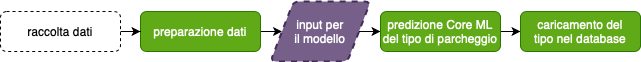
\includegraphics[width=14cm]{images/flow_diagram_predizione_tipo.png}
    \caption{Diagramma di flusso della predizione del tipo di parcheggio.}
    \label{fig:flow_diagram_predizione_tipo}
\end{figure}


\subsubsection{Caricamento etichetta ML nel database}

Successivamente alla predizione del tipo di parcheggio, quest'ultimo può essere salvato
nel database. Il caricamento avviene in maniera simile a quella in cui viene salvato il 
tipo ottenuto dalla notifica mostrata all'utente, attraverso la chiamata di una API del 
backend di GeneroCity. Tuttavia, è stato deciso di non confondere i due tipi (quello
selezionato dall'utente e quello ottenuto attraverso la predizione di ML), sovrascrivendo
l'uno con l'altro, bensì di creare due campi diversi per distinguere i due concetti
all'interno del database. Dopotutto, l'utilità del tipo selezionato dall'utente è proprio
quella di essere utilizzato nel dataset di training per addestrare il modello e portarlo 
al punto di essere in grado di classificare autonomamente il tipo di parcheggio stesso
con buona accuratezza.
Tra i motivi per cui si è scelto di non confondere i due valori ci sono:
\begin{itemize}
    \item non avrebbe più senso effettuare il training utilizzando un dataset in cui sono
    presenti dati classificati dal modello stesso.
    \item mantenendo i valori separati, si possono fare statistiche sul miglioramento
    (o peggioramento) dell'accuratezza del modello, all'aumentare della dimensione del
    dataset. Infatti, si può controllare la percentuale dei tipi classificati correttamente,
    comparandoli alle etichette selezionate dagli utenti.
    \item si possono fare studi sul comportamento del modello, capendo in che situazioni
    commette più errori e quali sono invece i suoi punti più stabili.
\end{itemize}
Oltre all'etichetta, viene caricato nel database anche il valore dell'heading 
precedentemente calcolato.










